\documentclass[11pt]{article}

\usepackage[margin=1in]{geometry}
\usepackage[T1]{fontenc}
\usepackage{lmodern}
\usepackage{microtype}
\usepackage{amsmath,amssymb,bm}
\usepackage{booktabs}
\usepackage{tabularx}
\usepackage{graphicx}
\usepackage{xcolor}
\usepackage{tikz}
\usetikzlibrary{positioning,arrows.meta,fit}
\usepackage[numbers,sort&compress]{natbib}
\usepackage[colorlinks=true,linkcolor=blue!60!black,citecolor=blue!60!black,urlcolor=blue!60!black]{hyperref}

\newcommand{\code}[1]{\texttt{#1}}

\title{BRIDGE: Question-Conditioned Graph Neural Retrieval for\\Question Answering over Building Knowledge Graphs}
\author{Project Proposal}
\date{}

\begin{document}
\maketitle
\vspace{-2em}

%==============================================================================
\section{Motivation}
%==============================================================================

Modern buildings collect an unprecedented volume of operational data. Building automation systems log thousands of sensor, setpoint, and command streams from HVAC, lighting, and metering equipment, often at minute-level resolution. In principle, these data could support data-driven solutions, such as fault detection and diagnosis, predictive maintenance, and optimized control, that reduce operating costs, energy use, and occupant discomfort.

In practice, however, these solutions rarely move beyond individual pilot projects. The main obstacle is not a lack of data but a lack of context: point names are vendor-specific and inconsistent, so every deployment first requires an expert to map manually \emph{which} sensor is attached to \emph{which} piece of equipment and serves \emph{which} space~\cite{pritoni2021metadata}.

Semantic graph models were introduced to remove this bottleneck. Ontologies such as Brick~\cite{balaji2016brick} and ASHRAE~223P~\cite{ashrae223p} describe a building as a knowledge graph (KG). In such a graph, equipment, spaces, and data points are linked by standardized, typed relations such as \code{feeds} and \code{hasPoint}, so that an application can locate the data it needs in any building through a single query.

Yet even where such graphs exist, they remain largely unused by the people who operate buildings. Retrieving information from a KG requires writing SPARQL queries over an unfamiliar ontology, a skill that facility managers and operators rarely possess~\cite{ko2026brickqa,mulayim2025buildingqa}. As a result, the value of both the operational data and the semantic models built to organize them goes largely unrealized. Knowledge graph question answering (KGQA), which translates a natural-language question into an executable query, offers a direct way to close this gap.

KGQA methods developed for open-domain graphs transfer poorly to this setting: on the BuildingQA benchmark, the strongest general-purpose agents attain a Row-Matching F1 of only $0.38$~\cite{mulayim2025buildingqa}. Building KGs differ from open-domain KGs in four respects:
\begin{enumerate}
  \item they use a specialized vocabulary and opaque identifiers (e.g., \code{AHU\_1\_SAT});
  \item answering a question typically requires multi-hop traversal of a dense, highly repetitive topology (e.g., sensor $\rightarrow$ VAV $\rightarrow$ zone);
  \item each building is modeled differently, and Brick and 223P employ different relation vocabularies;
  \item per-building training data are unavailable, so a method must generalize to buildings it has never seen.
\end{enumerate}

Domain-specific LLM agents have since raised the state of the art to $0.59$ Row-F1. BrickQA, our prior work, relies on dynamic graph exploration~\cite{ko2026brickqa}; BSchema relies on precomputed structural summaries~\cite{bschema2026}. Both systems are zero-shot and contain no learned graph component. Their residual errors are dominated by \emph{graph grounding}: vocabulary hallucination accounts for 79\% of failed queries, and topological mismatch, i.e., assuming a direct edge where the building uses a multi-hop path, for a further 16\%~\cite{bschema2026}.

These are precisely the decisions a graph neural network (GNN) can learn: which nodes, relations, and paths in a given graph are relevant to a given question.

GNNs are well suited to this role. In a building KG, relevance is determined by structure rather than by surface text: whether a sensor matters for a question about a zone depends on the chain of equipment that connects them, not on the sensor's opaque label. Message passing propagates information along exactly these relational chains, so a GNN can learn how each building realizes a concept topologically, which an LLM can only guess from the ontology. Moreover, a GNN trained across many buildings learns modeling patterns that recur from building to building, whereas a zero-shot LLM agent must rediscover them in every new graph.

Two recent developments make such learning feasible. First, Build2SPARQL now provides roughly 200 buildings and 30k question--query pairs~\cite{jung2026build2sparql}. Second, inductive GNNs can transfer to unseen graphs and unseen relation types~\cite{zhu2021nbfnet,galkin2024ultra}. We therefore propose \textbf{BRIDGE} (\textbf{B}uilding \textbf{R}etrieval via \textbf{I}nductive, \textbf{D}omain-general \textbf{G}raph \textbf{E}ncoding), which trains a question-conditioned GNN retriever on many buildings and uses it to ground LLM-based KGQA on unseen ones.

%==============================================================================
\section{Application Domain}
%==============================================================================

\subsection{Datasets}

We use three public resources (Table~\ref{tab:data}).
\begin{itemize}
  \item \textbf{Build2SPARQL}~\cite{jung2026build2sparql} is used for training and in-distribution testing. It contains 201 buildings (180 Brick, 21 ASHRAE 223P) with 6{,}136 executable SPARQL queries spanning six structural patterns. Each query is paired with five natural-language paraphrases of increasing abstraction, for a total of 30{,}680 questions.
  \item \textbf{Source building graphs.} Queries are executed against these graphs, which are drawn from Mortar~\cite{fierro2019mortar}, the Brick reference models, the open223 models, and BuildGraph.
  \item \textbf{BuildingQA}~\cite{mulayim2025buildingqa} serves as the final held-out benchmark. It comprises 188 expert-derived questions over four real buildings (three Brick, one 223P), with queries of up to 53 triple patterns and 16 projected variables.
\end{itemize}

\begin{table}[h]
\centering
\small
\caption{Datasets used in this project. All are publicly available.}
\label{tab:data}
\begin{tabularx}{\linewidth}{@{}l X l@{}}
\toprule
Dataset & Content & Availability \\
\midrule
Build2SPARQL v1.0~\cite{jung2026build2sparql} & 201 buildings; 6{,}136 queries; 30{,}680 questions & Zenodo (CC BY-NC 4.0) \\
Source building graphs & Mortar, Brick examples, open223, BuildGraph & Public repositories \\
BuildingQA~\cite{mulayim2025buildingqa} & 4 buildings; 27 expert queries; 188 questions & GitHub \\
\bottomrule
\end{tabularx}
\end{table}

\paragraph{Leakage-free split.}
The split released with Build2SPARQL places exact duplicate buildings (e.g., \code{HPL} and \code{NIST-HPL}) on both sides of the train/test boundary, so we construct our own split. Specifically, we:
\begin{enumerate}
  \item remove the building that also appears in BuildingQA, together with exact duplicates;
  \item group near-duplicate buildings (query-signature Jaccard similarity $\geq 0.8$) and buildings from the same source family;
  \item assign whole groups to splits, stratified by ontology and corpus.
\end{enumerate}
No near-duplicate pair crosses the resulting splits (Table~\ref{tab:split}). The test set contains six 223P buildings from three independent families and one held-out synthetic building type. Both source datasets are already public, and before submission we will release the split, its generation script, the executed gold answers, the derived supervision labels, and all code.
% TODO: if the hand-modeled real office building is used as a case study, confirm that an (anonymized) release is possible; otherwise exclude it from reported results.

\begin{table}[h]
\centering
\small
\caption{Building-level split of Build2SPARQL used in this project.}
\label{tab:split}
\begin{tabular}{@{}lrrrl@{}}
\toprule
Split & Buildings & Queries & Questions & Notes \\
\midrule
Train      & 154 & 4{,}670 & 23{,}350 & -- \\
Validation &   9 &     256 &  1{,}280 & real buildings only \\
Test       &  33 & 1{,}012 &  5{,}060 & 6 ASHRAE 223P buildings; one unseen building type \\
\bottomrule
\end{tabular}
\end{table}

\subsection{Task and Metrics}

Let $G=(\mathcal{V},\mathcal{R},\mathcal{E})$ denote a building KG with entities $\mathcal{V}$, relation types $\mathcal{R}$, and typed edges $\mathcal{E}\subseteq\mathcal{V}\times\mathcal{R}\times\mathcal{V}$, and let $q$ be a natural-language question. The end task is to produce a SPARQL query whose execution on $G$ yields the correct answer table.

Our graph learning task is \emph{question-conditioned retrieval}. The model assigns a relevance score to every node $v\in\mathcal{V}$ and every edge $(u,r,v)\in\mathcal{E}$, and returns the top-$k$ relational paths, which an LLM then composes into SPARQL. Supervision is obtained by execution rather than by annotation: binding the variables of each gold query identifies its evidence nodes, edges, and class-level paths, which yields approximately 23k labeled (question, subgraph) pairs.

\paragraph{Retrieval metrics.} On the Build2SPARQL test split we report recall@$k$ of evidence nodes and edges, hit@$k$ of the gold path, schema-linking F1, and context size.

\paragraph{End-to-end metrics.} On BuildingQA we use the official metrics. After aligning the columns of the predicted table $P$ to those of the gold table $T$ by the best permutation, \emph{Row-Matching F1} is the harmonic mean of row precision $|P\cap T|/|P|$ and row recall $|P\cap T|/|T|$; this is our primary metric. We additionally report Entity-Set F1, Exact-Match F1, and Arity F1.

\paragraph{Rationale.} These datasets suit graph learning for four reasons:
\begin{itemize}
  \item every building is a distinct graph, so the task directly evaluates inductive generalization;
  \item Brick and 223P have largely disjoint relation vocabularies, which tests transfer to unseen relation types;
  \item execution provides exact subgraph-level supervision at no annotation cost;
  \item BuildingQA offers a challenging, expert-written benchmark with established baselines.
\end{itemize}

%==============================================================================
\section{Graph ML Techniques}
%==============================================================================

\subsection{Model}

We build on conditional message passing, as introduced in NBFNet~\cite{zhu2021nbfnet} and generalized to fully inductive reasoning in ULTRA~\cite{galkin2024ultra}. We adapt it to natural-language queries and path retrieval, following GNN-RAG~\cite{mavromatis2025gnnrag} and SubgraphRAG~\cite{li2025subgraphrag}. Figure~\ref{fig:model} summarizes the architecture.

\begin{figure}[h]
\centering
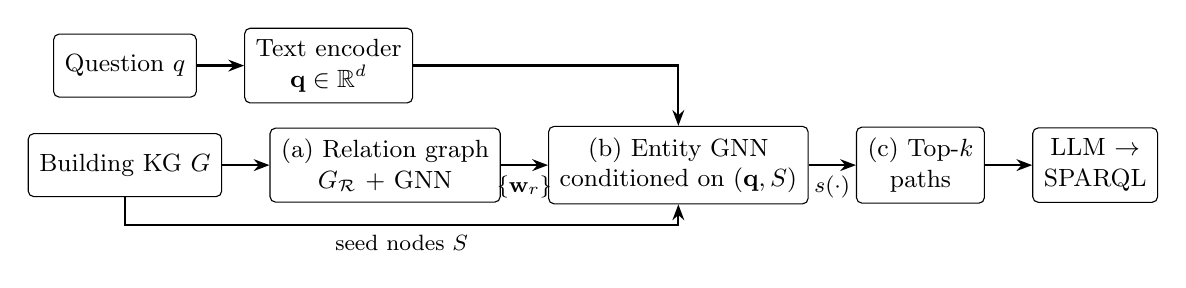
\begin{tikzpicture}[
  font=\small,
  box/.style={draw, rounded corners=2pt, align=center, minimum height=0.8cm, inner sep=4pt},
  arr/.style={-{Stealth[length=2mm]}, thick},
  node distance=0.45cm and 0.6cm]
  \node[box] (q) {Question $q$};
  \node[box, right=of q] (enc) {Text encoder\\$\mathbf{q}\in\mathbb{R}^d$};
  \node[box, below=of q] (kg) {Building KG $G$};
  \node[box, right=of kg] (rg) {(a) Relation graph\\$G_{\mathcal{R}}$ + GNN};
  \node[box, right=of rg] (ent) {(b) Entity GNN\\conditioned on $(\mathbf{q},S)$};
  \node[box, right=of ent] (path) {(c) Top-$k$\\paths};
  \node[box, right=of path] (llm) {LLM $\rightarrow$\\SPARQL};
  \draw[arr] (q) -- (enc);
  \draw[arr] (kg) -- (rg);
  \draw[arr] (rg) -- node[below, font=\footnotesize]{$\{\mathbf{w}_r\}$} (ent);
  \draw[arr] (enc) -| (ent);
  \draw[arr] (ent) -- node[below, font=\footnotesize]{$s(\cdot)$} (path);
  \draw[arr] (path) -- (llm);
  \draw[arr] (kg.south) -- ++(0,-0.35) -| node[pos=0.25, below, font=\footnotesize]{seed nodes $S$} (ent.south);
\end{tikzpicture}
\caption{Overview of BRIDGE: question-conditioned GNN retrieval for building KGQA.}
\label{fig:model}
\end{figure}

\paragraph{(a) Relation graph.}
Following ULTRA, we construct a graph $G_{\mathcal{R}}$ whose nodes are the relation types of $G$. Two relations are connected by one of four meta-relations (head--head, head--tail, tail--head, tail--tail), according to how they share entities. A GNN on $G_{\mathcal{R}}$ produces an embedding $\mathbf{w}_r$ for each relation of the given building. Because no relation embedding table is learned, relations unseen during training, such as the 223P relation \code{connectedTo}, still receive representations.

\paragraph{(b) Question-conditioned entity GNN.}
Node states are pairwise with respect to the query and are computed by a generalized Bellman--Ford iteration. The question embedding is injected at a set of seed nodes $S$, obtained by linking the question to ontology classes and explicit mentions:
\begin{align}
  \mathbf{h}^{(0)}_q(v) &= \mathbb{1}[v\in S]\, \mathbf{W}_0\, \mathbf{q}, \label{eq:boundary}\\
  \mathbf{h}^{(t)}_q(v) &= \mathrm{LN}\Big(\mathrm{AGG}\big(\{\mathbf{h}^{(t-1)}_q(u)\odot\mathbf{w}^{(t)}_r : (u,r,v)\in\mathcal{E}\}\cup\{\mathbf{h}^{(0)}_q(v)\}\big)\Big) + \mathbf{h}^{(t-1)}_q(v). \label{eq:bf}
\end{align}
Messages follow DistMult, $\mathrm{AGG}$ is sum or PNA aggregation, and the residual term preserves the previous state. After $L$ layers (typically $4$--$6$), nodes and edges are scored as
\begin{equation}
  s(v)=\sigma\big(\mathrm{MLP}([\mathbf{h}^{(L)}_q(v);\mathbf{q}])\big),\qquad
  s(u,r,v)=\sigma\big(\mathrm{MLP}([\mathbf{h}^{(L)}_q(u);\mathbf{w}_r;\mathbf{h}^{(L)}_q(v)])\big).
\end{equation}

\paragraph{(c) Path retrieval.}
From the top-$k$ nodes ranked by $s(v)$, we extract the highest-scoring paths from the seed nodes by beam search, scoring each path by the sum of its log edge scores. The selected paths are lifted to the class level (e.g., \code{VAV}~$\xrightarrow{\text{feeds}}$~\code{HVAC\_Zone}) and verbalized as context for the LLM.

\paragraph{Training.}
We minimize
\begin{equation}
  \mathcal{L}=\mathcal{L}^{\text{node}}_{\text{BCE}}+\mathcal{L}^{\text{edge}}_{\text{BCE}}+\lambda\,\mathcal{L}_{\text{path}}.
\end{equation}
The two binary cross-entropy terms are supervised by the execution-derived evidence labels. $\mathcal{L}_{\text{path}}$ is a contrastive loss that uses the gold class-level path as the positive and sibling paths sharing its endpoints as hard negatives. We optionally warm-start the model with ULTRA-style link-prediction pretraining over all building graphs. The implementation uses PyTorch Geometric.

\paragraph{Baselines and ablations.}
We compare against several retrievers at an equal context budget:
\begin{itemize}
  \item text-embedding nearest neighbors over triples;
  \item prize-collecting Steiner tree (PCST) subgraph selection from G-Retriever~\cite{he2024gretriever};
  \item an R-GCN node classifier~\cite{schlichtkrull2018rgcn};
  \item the SubgraphRAG triple scorer~\cite{li2025subgraphrag};
  \item static BSchema summaries~\cite{bschema2026}.
\end{itemize}
Our ablations replace the relation graph with learned relation embeddings, remove the query conditioning, and remove the path loss.

\subsection{Suitability of the Model for the Data}

\paragraph{Inductive over entities and relations.}
NBFNet and ULTRA learn no entity embeddings and therefore apply, by construction, to unseen buildings, where transductive KG embeddings such as TransE~\cite{bordes2013transe} and RotatE~\cite{sun2019rotate} cannot. ULTRA additionally derives relation representations from structure. A model trained predominantly on Brick can thus transfer to 223P, which is the most difficult BuildingQA building: the best reported Row-F1 there is $0.30$.

\paragraph{Expressivity on repetitive graphs.}
Building KGs repeat the same motif (e.g., VAV--zone--sensor) thousands of times. Standard message passing is bounded by the 1-WL test~\cite{xu2019gin}, so it assigns identical representations to structurally identical nodes and cannot distinguish \emph{which} VAV a question refers to. Conditional message passing acts as a labeling trick: it computes representations relative to the question's seed nodes, which is provably more expressive for query-dependent prediction~\cite{huang2023relationalwl}. The current state of the art, BSchema, is in effect a non-learned, question-agnostic 1-WL color refinement; our model can be viewed as its learned, question-conditioned counterpart.

\paragraph{Alignment with the downstream task.}
SPARQL queries are compositions of relational paths, and topological mismatch is fundamentally a path error. A model that scores and returns paths therefore targets the dominant failure mode directly.

\paragraph{Scalability.}
Model size is independent of graph size. The per-question cost is $\mathcal{O}(L\,|\mathcal{E}|\,d)$ and can be further reduced by restricting message passing to a $k$-hop neighborhood of the seed nodes.

\bibliographystyle{plainnat}
\bibliography{references}

\end{document}
